\section{Configuración técnica - Copia de seguridad}
\subsection{Autoevaluación}
En esta sección se han cumplido los objetivos correspondientes al 10.
\subsection{Introducción}
\paragraph{}
Este apartado aborda la gestión de las copias de seguridad en Odoo. Se va a hacer una evaluación de la configuración que ofrece para gestionar las bases de datos, la posibilidad de transferir los datos de Odoo de una instancia a otra y la capacidad de crear scripts para automatizar las copias de seguridad, las cuáles van a ser almacenadas en la nube.
\subsection{Metodología}
\paragraph{}
El primer paso que se ha realizado ha sido dirigirnos a la siguiente dirección en el navegador:\\ \href{http://ec2-13-51-201-201.eu-north-1.compute.amazonaws.com:8069/web/database/manager}{http://ec2-13-51-201-201.eu-north-1.compute.amazonaws.com:8069/web/database/manager}. Se ha hecho click en \textit{Set Master Password} y se ha introducido una contraseña que será necesaria en las operaciones que se van a realizar en este módulo.
\paragraph{}
A continuación, Odoo ofrece una opción para crear una nueva base de datos, para ello se ha hecho click en \textit{Create Database} y se ha rellenado el formulario. Tras pulsar el botón de crear hay que esperar hasta que nos ha redirigido al inicio de sesión, una vez iniciado sesión con la información introducida anteriormente, ya puedes acceder a Odoo. 
\paragraph{}
También, ofrece una opción para duplicar una base de datos, para ello se ha pulsado en \textit{Duplicate} en la base de datos que se quiere duplicar y se ha introducido el nuevo nombre y la contraseña maestra, tras unos segundos se ha comprobado que se ha mostrado una nueva entrada en la lista de bases de datos, la cual tendrá la misma información que la original.
\paragraph{}
Odoo nos da la posibilidad de eliminar bases de datos. En la lista se ha pulsado el botón \textit{Delete} del elemento que se quiere borrar y tras introducir la contraseña maestra se ha eliminado la base de datos. Por último, Odoo ofrece la posibilidad de realizar una copia de seguridad de las bases de datos. Para probar esta funcionalidad se ha hecho clic en \textit{Backup} en la base de datos que se quiere realizar y se ha seleccionado el formato zip. Cómo resultado se descarga en la máquina un zip con la información de la base de datos. 
\paragraph{}
La capacidad de exportar la información junto con la posibilidad que ofrece Odoo de restaurar una base de datos, nos permite realizar transferencias de las bases de datos. Para comprobarlo se ha hecho una copia de seguridad de una de ellas como se ha explicado anteriormente y se ha enviado por WhatsApp. En otra máquina donde se tiene instalado Odoo, se ha accedido a WhatsApp y se ha descargado el zip. A continuación, hemos abierto en nuestro navegador la instancia de odoo localmente y nos hemos dirigido a \textit{http://localhost:8069/web/database/manager} y se ha hecho click en \textit{Restore Database}, se ha introducido la contraseña maestra y el nombre, se ha activado la opción de que la base de datos es una copia y se ha seleccionado el zip que contiene la información. Como resultado se ha creado una nueva entrada en la lista de bases de datos la cual contiene la información que se tenía en la otra máquina.

\paragraph{}
Los pasos descritos nos permiten realizar la copia de seguridad de forma manual, sin embargo, creemos que esto no es viable para una empresa. Esta tarea se debe automatizar asegurándonos su correcto funcionamiento. Para ello hemos realizado el siguiente script en nuestra máquina remota:

\begin{lstlisting}[frame=single, basicstyle=\tiny]
#!/bin/bash
# vars
BACKUP_DIR=/home/ubuntu/sisInfo2_proyect/backups
ODOO_DATABASE=GOOD
ADMIN_PASSWORD=adminadmin

# create a backup directory
mkdir -p ${BACKUP_DIR}

# create a backup
curl -X POST \
    -F "master_pwd=${ADMIN_PASSWORD}" \
    -F "name=${ODOO_DATABASE}" \
    -F "backup_format=zip" \
    -o ${BACKUP_DIR}/${ODOO_DATABASE}.$(date +%F_%H-%M-%S).zip \
    http://localhost:8069/web/database/backup

# push to github
cd /home/ubuntu/sisInfo2_proyect
git pull
git add .
git commit -m "backup $(date +%F_%H-%M-%S)"
git push
\end{lstlisting}

\paragraph{}
En este script hecho con \textit{Bash} lo primero que hacemos es definir las variables, facilitando cualquier posible cambio de nombre o ruta en un futuro. A continuación se realiza la copia de seguridad y se almacena en el directorio definido anteriormente. Por último, se hace un commit a un repositorio de Github donde se encuentran todas las copias de seguridad realizadas. De esta forma tenemos almacenadas todas nuestras copias de seguridad en un lugar distinto a nuestra máquina remota. Por tanto, conseguimos que en caso de cualquier imprevisto tenemos una copia de seguridad alejada físicamente de nuestro sistema funcional. Cabe destacar que para poder realizar el commit desde la máquina remota se ha tenido que clonar el repositorio y permitir realizar commits. Para ello hemos utilizado la herramienta que nos proporciona Github; \href{https://docs.github.com/es/github-cli/github-cli/quickstart}{GitHub CLI}. 
\paragraph{}
El segundo paso en el proceso de automatizar esta tarea es ejecutar este script de forma regular y automática. Para ello, hemos creado un demonio que se encarga de ejecutarlo cada día a la una de la madrugada. Para ello hemos ejecutado el siguiente comando:
\begin{lstlisting}[frame=single, basicstyle=\tiny]
crontab -e
\end{lstlisting}
\paragraph{}
Y con el editor de texto añadimos la siguiente línea:
\begin{lstlisting}[frame=single, basicstyle=\tiny]
0 1 * * * /home/ubuntu/script.sh
\end{lstlisting}
\paragraph{}
Con esta línea indicamos que a la 1:00 de cada día se ejecuta el script que se encuentra en esa dirección, por lo tanto, en caso de cambiar de lugar el script se debería modificar esa línea también.

\subsection{Resultados y análisis}
Se ha conseguido realizar en Odoo la creación, eliminación, duplicación y copia de seguridad de una base de datos. Además, se ha conseguido transferir una base de datos de una instancia de Odoo a otra, mediante realización de una copia de seguridad de una base de datos y la restauración de la misma. Por último hemos conseguido automatizar esta tarea, creando un script, generando un demonio en nuestra máquina remota y almacenándolas en una lugar físico distinto a la máquina remota. Como lugar de almacenamiento remoto hemos elegido Github, como hemos comentado previamente. Esta decisión se ha basado en la facilidad de subir las copias de seguridad, el control de versiones y que podemos acceder desde cualquier lugar con conexión, ya que el repositorio donde la estamos almacenando es público. El control de versiones nos permite en todo momento acceder a la versión de cualquier día. Si observamos el historial de commits de \href{https://github.com/Practicass/sisInfo2_proyect/commits/main/}{nuestro repositorio} podemos recuperar cualquier copia de seguridad. 
\newpage
\begin{figure}[h]
    \centering
    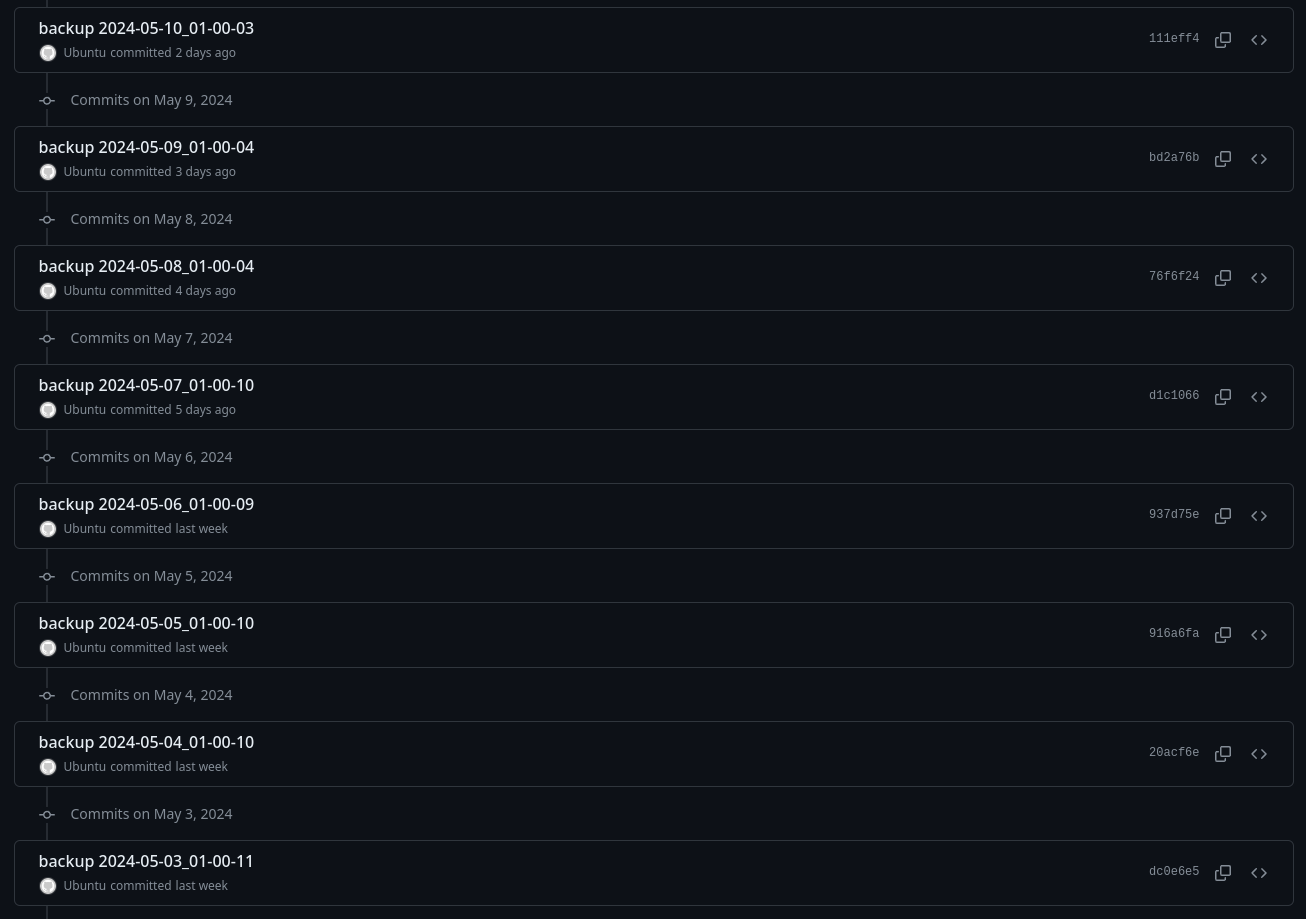
\includegraphics[width=1\linewidth]{backup/commits.png}
    \caption{Historial de commits del repositorio}
\end{figure}
\subsection{Conclusiones}
En esta sección hemos analizado como se puede realizar la copia de seguridad de nuestro ERP. Odoo tiene sistema de backup muy sencillo e intitutivo. Que nos permite tener en todo momento nuestra base de datos replicada. Consideramos que es fundamental que estas \textit{backups} no se encuentren en el mismo lugar físico que la base de datos, ya que en caso de una catástrofe como puede ser un incendio de los servidores en los que tenemos nuestra base de datos, en nuestro caso, los servidores de AWS de Estocolmo; perderíamos todo. En cambio, al tener las copias de seguridad en un lugar físico tendríamos la capacidad de recomponer el sistema en minutos.

\paragraph{}
Además tener copias de seguridad no solo nos previene de catástrofes inesperadas, también de nuestros errores. Durante las últimas semanas de elaboración de este análisis cometimos un error que nos causo problemas y no conseguíamos deshacer los pasos que habíamos realizado. Es por ello, que tomamos la decisión de volver a una versión antigua y utilizar una de las copias de seguridad que se habían realizado.
\newpage
\section{Configuración técnica - Correo electrónico}
\label{sec:correo}
\subsection{Autoevaluación}
8
\subsection{Introducción}
Con el objetivo de permitir la comunicación de la empresa mediante Odoo se ha configurado un servidor de correo electrónico tanto saliente para poder enviar correos como entrante para poder recibirlos.
\subsection{Metodología}
Para crear un servidor SMTP y poder enviar correos a través de él, hay que ir a los ajustes de opciones generales, entrar en el menú de Servidores de correo saliente y crear un nuevo servidor. En este caso, se ha utilizado autentificación OAuth de Gmail, hay que asegurarse que se ha introducido \textit{odoo.com} en el campo Filtro DESDE, TLS como encriptación, \textit{smtp.gmail.com} como servidor SMTP y puerto 587. Se ha creado un correo para llevar a cabo la conexión con Gmail por lo que se ha puesto ese correo en el campo de nombre de usuario. A continuación, hay que insertar el ID y el Numero secreto en \textit{Usar un servidor de Gmail} en las opciones generales de los ajustes. Para ello, se ha ido a la siguiente web \href{https://console.cloud.google.com/apis/}{https://console.cloud.google.com/apis/} se ha iniciado sesión en Gmail y se ha creado un nuevo proyecto llamado Odoo. Primero, en pantalla de consentimiento de OAuth se ha elegido el tipo de usuario externo, se han rellenado los formularios necesarios, cabe destacar que hay que añadir como dominio autorizado \textit{odoo.com}. A continuación, se ha ido al menú \textit{Crear credenciales} y se ha seleccionado la opción OAuth client ID. En este menú se ha elegido la opción \textit{Aplicación web} y se ha añadido como URIS de redirección autorizadas \textit{http://ec2-13-51-201-201.eu-north-1.compute.amazonaws.com:8069/google\_gmail/confirm} . En la misma pantalla se mostrará el \textit{ID} y \textit{Secreto} con los que hay que rellenar los campos en Odoo. En la pantalla del servidor de correo que se estaba creando la prueba de conexión será exitosa. Por otro lado, el proceso de añadir un servidor de correo entrante es similar. Cabe destacar que en el campo de nombre del servidor se ha introducido \textit{imap.gmail.com} y se ha activado la opción SSL/TLS. Además, hay que ir a los ajustes de Gmail y habilitar IMAP, desde el apartado \textit{Reenvío e IMAP/POP}. Para llevar a cabo el proceso de envío de un correo electrónico desde Odoo y probar el servidor de salida se ha instalado el módulo Contactos. En este módulo se muestra todos los contactos de empleados, empresas, individuos que se ha tenido. Si se hace click en un contacto, se podrá ver a la derecha un chat en el que se ha escrito un correo y se ha enviado. Además, si se produce una respuesta a ese correo aparecerá en el mismo chat. 
\subsection{Resultados y análisis}
Se ha conseguido configurar un servidor SMTP mediante Gmail y autentificación OAuth de Gmail. Se ha realizado el envío de un correo electrónico desde Odoo mediante el servidor de correo saliente.
\newpage
\begin{figure}[h]
    \centering
    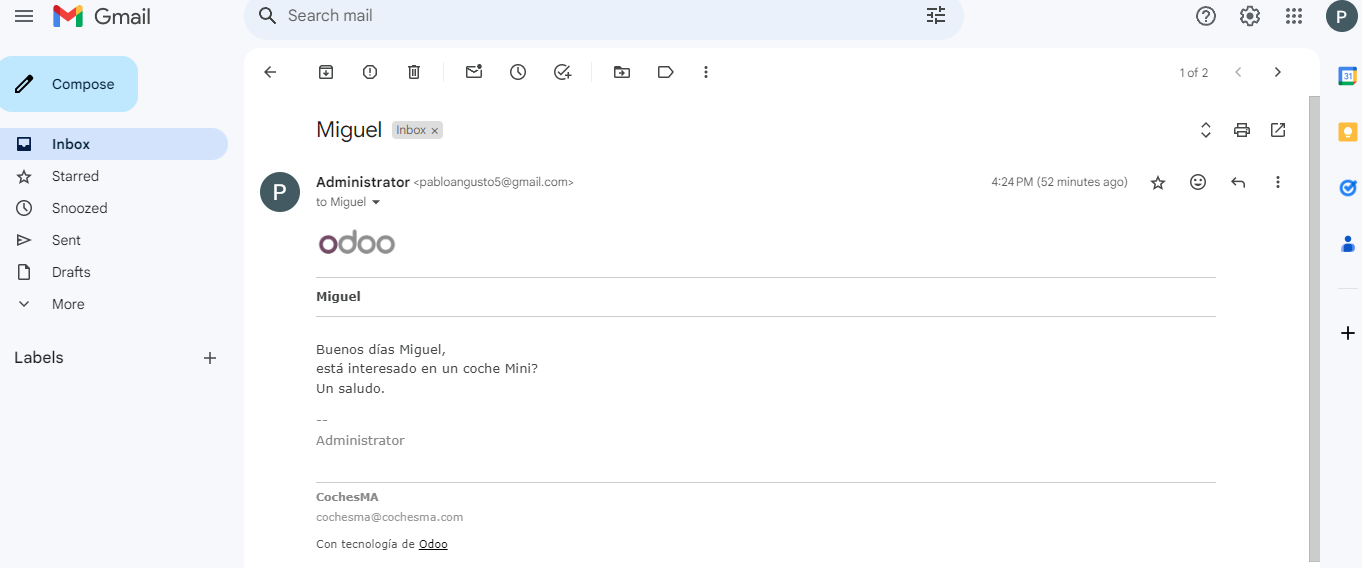
\includegraphics[width=1\linewidth]{fotosConfiguración/correoEnvio1.png}
    \caption{Correo saliente desde bandeja de salida}
    \label{fig:enter-label}
\end{figure}
Además, se ha comprobado el correcto funcionamiento del servidor de correo entrante como se muestra en la siguiente figura.
\begin{figure}[h]
    \centering
    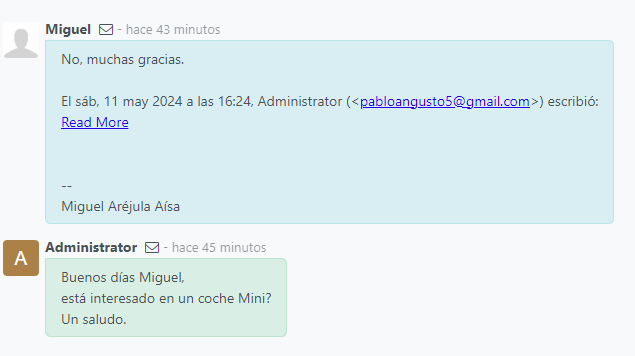
\includegraphics[width=1\linewidth]{fotosConfiguración/correoOdoo.png}
    \caption{Conversación de correos desde Odoo}
    \label{fig:enter-label}
\end{figure}
Por último, se examinaron las capacidades de automatización de Odoo en relación con la gestión de correos electrónicos. Esta funcionalidad específica de Odoo se encuentra disponible a través del módulo \textit{Studio}, el cual no está habilitado en la versión de Docker de Odoo, sino únicamente en la versión en la nube. Mediante este módulo, es posible establecer reglas que se activan en función de eventos internos del sistema o de los correos electrónicos recibidos por el sistema.
Cabe destacar qué en el modulo de \textit{Ventas} existe una funcionalidad similar a la del módulo Studio, que permite generar iniciativas a partir de correos pero no cubre los requisitos planteados.
\subsection{Conclusiones}
\paragraph{}
La configuración y gestión de correos electrónicos en Odoo se muestran como procesos accesibles y bien estructurados, lo que permite una integración eficiente con proveedores externos como Google y una comunicación fluida dentro de la plataforma.
\paragraph{}
Las configuraciones que se han realizado en este módulo, son algo complejas, en especial si nunca se ha utilizado una cuenta de Gmail para realizar este tipo de funcionalidades. Además, requiere configuraciones fuera de Odoo tanto en Google Cloud como en Gmail esto añade dificultad a la hora de realizar este módulo. Sin embargo, es una tarea que resulta importante porque tiene un gran impacto en la comunicación de la compañía. Mediante la configuración del servidor saliente SMTP y el servidor entrante IMAP de manera precisa se garantiza una comunicación adecuada con el servicio de correo. Una vez configurados los servidores de correo, Odoo permite enviar y recibir mensajes directamente desde la plataforma, simplificando así la gestión de la comunicación interna y externa de la empresa.
\paragraph{}
Es importante destacar que la configuración del servidor de correo entrante IMAP puede presentar algunos problemas, ya que se ha realizado este proceso con los correos de UNIZAR y no ha tenido un correcto funcionamiento por lo que habría que tener presente esta posibilidad con los correos de empresa y que igual implica alguna configuración más.
\paragraph{}
En cuanto a las capacidades de automatización, aunque se puedan implementar con alguna solución en local están limitadas a usar el módulo \textit{Studio} de la versión en la nube. Permite acciones específicas en función de eventos internos del sistema o correos electrónicos recibidos, aunque no está disponible en la versión de Docker.








